\documentclass[10pt]{beamer}
\title[$E_r$-Generating Mechanisms in L-H Transitions]{Comparing Radial Electric Field-Generating Mechanisms in L--H Transitions}
\author[K.A. Blondino]{
\includegraphics[height=1.5cm]{../Graphics/tue_fusion_logo.png} \\ Kevin A. Blondino \\
	Supervisor: dr. H.J. de Blank, TU/e \& DIFFER}
\institute[TU/e]{Eindhoven University of Technology \\
	\medskip
	\textit{k.blondino@student.tue.nl}}
\date{\today}

%{{{ Presentation Style and Color
\mode<presentation>
{
%\usetheme{default}
%\usetheme{AnnArbor}
%\usetheme{Antibes}
%\usetheme{Bergen}
%\usetheme{Berkeley}
\usetheme{Berlin}
%\usetheme{Boadilla}
%\usetheme{CambridgeUS}
%\usetheme{Copenhagen}
%\usetheme{Darmstadt}
%\usetheme{Dresden}
%\usetheme{Frankfurt}
%\usetheme{Goettingen}
%\usetheme{Hannover}
%\usetheme{Ilmenau}
%\usetheme{JuanLesPins}
%\usetheme{Luebeck}
%\usetheme{Madrid}
%\usetheme{Malmoe}
%\usetheme{Marburg}
%\usetheme{Montpellier}
%\usetheme{PaloAlto}
%\usetheme{Pittsburgh}
%\usetheme{Rochester}
%\usetheme{Singapore}
%\usetheme{Szeged}
%\usetheme{Warsaw}

%\usecolortheme{albatross}
\usecolortheme{beaver}
%\usecolortheme{beetle}
%\usecolortheme{crane}
%\usecolortheme{dolphin}
%\usecolortheme{dove}
%\usecolortheme{fly}
%\usecolortheme{lily}
%\usecolortheme{orchid}
%\usecolortheme{rose}
%\usecolortheme{seagull}
%\usecolortheme{seahorse}
%\usecolortheme{whale}
%\usecolortheme{wolverine}

%\setbeamertemplate{caption}[numbered]
\setbeamertemplate{bibliography item}{\insertbiblabel}
%\setbeamertemplate{footline} % To remove the footer line in all slides uncomment this line
%\setbeamertemplate{footline}[page number] % To replace the footer line in all slides with a simple slide count uncomment this line

%\setbeamertemplate{navigation symbols}{} % To remove the navigation symbols from the bottom of all slides uncomment this line
}
%}}}

%{{{ Packages
\usepackage{amsmath,graphicx,booktabs,moresize,textpos}
\usepackage[utf8]{inputenc}
\usepackage{caption}
\captionsetup{labelfont=bf}
\usepackage[UKenglish]{isodate}
\cleanlookdateon
%}}}

% SageTeX!
\usepackage{sagetex}

%{{{ Setup References
\usepackage[backend=bibtex, style=authoryear]{biblatex}
\addbibresource{../References/References.bib}
\renewcommand*{\nameyeardelim}{\addcomma\addspace}
%}}}

%{{{ Two Figures Side-by-Side, separate captions
%\newsavebox\IBoxA \newsavebox\IBoxB \newlength\IHeight
\newcommand\TwoFig[6]{% Image1 Caption1 Label1 Im2 Cap2 Lab2
%	\sbox\IBoxA{#1}
%	\sbox\IBoxB{#4}%
%	\ifdim\ht\IBoxA>\ht\IBoxB
%		\setlength\IHeight{\ht\IBoxB}%
%	\else\setlength\IHeight{\ht\IBoxA}\fi
	\begin{figure}[hbt]
		\minipage[t]{0.48\textwidth}\centering
			{#1}
			\caption{#2}\label{#3}
		\endminipage\hfill\vrule\hfill
		\minipage[t]{0.48\textwidth}\centering
			{#4}
			\caption{#5}\label{#6}
		\endminipage
	\end{figure}%
}
%}}}

%{{{ Two Figures Side-by-Side, with 1 caption
\newcommand\TwoFigOneCap[4]{% Image1 Im2 Caption Label
%	\sbox\IBoxA{#1}
%	\sbox\IBoxB{#2}%
%	\ifdim\ht\IBoxA>\ht\IBoxB
%		\setlength\IHeight{\ht\IBoxB}%
%	\else\setlength\IHeight{\ht\IBoxA}\fi
	\begin{figure}[hbt]
		\minipage[t]{0.48\textwidth}\centering
			{#1}
		\endminipage\hfill
		\minipage[t]{0.48\textwidth}\centering
			{#2}
		\endminipage
		\caption{#3}\label{#4}
	\end{figure}%
}
%}}}

\begin{document}
\begin{frame} % Title page
\setcounter{framenumber}{0}
\titlepage
\end{frame}

\addtobeamertemplate{frametitle}{}
{
\begin{textblock*}{100mm}(0.85\textwidth,-1cm)
	
\includegraphics[height=1cm,width=2cm]{../Graphics/tue_fusion_logo.png}
\end{textblock*}
}

\begin{frame} % Table of Contents
\setcounter{framenumber}{0}
\tableofcontents
\end{frame}

%--------------------------------------

\section{Bifurcation Theory}
\begin{sagesilent}
	reset()
	var('x,t,a,b')
		# ----------------- Co-dimension 1 ------------------------
	a_min, a_max = -1.5, 0.5
	x_min, x_max = -1.25, 1.25

	# Co-dimension 1 equation
	f1 = diff(x,t) == a + x^2

	co_1 = plot_vector_field((0, f1 / sqrt(a^2 + x^2)), (a, a_min, a_max), (x, x_min, x_max), color='blue', axes=True, frame=True)


	co_1_root = solve(a + x^2 == 0, x)
	co_1_lower = implicit_plot(co_1_root[0], (a,a_min,a_max), (x,x_min,x_max), linewidth=2.5, axes_labels=['$a$','$x$'], color='red', plot_points=2000, gridlines=False, fontsize=20, title="Co-dimension 1 Fold")
	co_1_upper = implicit_plot(co_1_root[1], (a,a_min,a_max), (x,x_min,x_max), linewidth=2.5, color='green', plot_points=2000, figsize=10, typeset='type1')

	# Zero point
	co_1_zero = point((0,0), size=30, color='black')

	co_1_total = co_1_lower + co_1_upper + co_1 + co_1_zero

	# ----------------- Co-dimension 2 ------------------------
	a_min, a_max = -1.2, 1.2
	x_min, x_max = -1.5, 1.5
	var('b')

	# Co-dimension 2 equation
	f2 = diff(x,t) == -(a + b*x - x^3).subs(b=1.1)

	co_2 = plot_vector_field((0, f2), (a, a_min, a_max), (x, x_min, x_max), color='blue', axes=True, frame=True)

	# Points
	turning_point_a = 1/3*sqrt(3)
	turning_point_x = solve(f2.subs(a=turning_point_a), x)[0].right().real()

	co_2_low = implicit_plot(f2.right() == 0, (a, a_min, a_max), (x, x_min, -turning_point_a), linewidth=2.5, color='green', axes_labels=['$a$','$x$'], axes=True, fontsize=20, title="Co-dimension 2 Fold")
	co_2_mid = implicit_plot(f2.right() == 0, (a, a_min, a_max), (x, -turning_point_a, turning_point_a), linewidth=2.5, color='red', axes=True)
	co_2_high = implicit_plot(f2.right() == 0, (a, a_min, a_max), (x, turning_point_a, x_max), linewidth=2.5, color='green', axes=True, figsize=10, typeset='type1')

	arrow_up = arrow((0.48, -0.55), (0.48, 1.2), width=3, color='black')
	arrow_down = arrow((-0.48, 0.55), (-0.48, -1.2), width=3, color='black')

	#co_2_zero1 = point((turning_point_a, turning_point_x), size=40, color='black')
	#co_2_zero2 = point((-turning_point_a, -turning_point_x), size=40, color='black')

	co_2_total = co_2 + co_2_low + co_2_mid + co_2_high + arrow_up + arrow_down
\end{sagesilent}
\begin{frame} % Bifurcation Theory, Co-dimension 1
\frametitle{Bifurcation Theory}
\begin{figure}[h]
\begin{minipage}{0.49\linewidth}
	\centering
	\sageplot[width=\linewidth]{co_1_total}
\end{minipage}
\begin{minipage}{0.49\linewidth}
	Bifurcation -- A topological or qualitative change in a system when a smooth change of parameter is made. \vspace*{5mm}
	\caption{Plot of steady-state of $\dot{x} \,=\, a \,+\, x^2$; red is unstable, green is stable}
\end{minipage}
\end{figure}

\end{frame}

%--------------------------------------

\begin{frame} % Co-dimension 2, Hysteresis
\frametitle{Bifurcation Theory}
\begin{figure}[h]
\begin{minipage}{0.49\linewidth}
	\centering
	\sageplot[width=\linewidth]{co_2_total}
\end{minipage}
\begin{minipage}{0.49\linewidth}
	Hysteresis -- the dependence of a state on the history of the system. \vspace*{5mm}
	\caption{Plot of steady-state of $\dot{x} \,=\, -(a \,+\, bx \,-\, x^3)$; red is unstable, green is stable}
\end{minipage}
\end{figure}
\end{frame}

%--------------------------------------

\begin{sagesilent} # SHOW ZEROS!
	reset()

	var('x, a, b, x_dot,t')
	x_min, x_max = -2.0, 2.0

	"""
		ROOT FINDING function, for all of the roots.
		Returns a sorted list of UNIQUE roots. This does NOT work when there
		is multiplicity in the roots. Use `w.roots()` to symbolically check
		for multiplicity.
	"""
	def find_root_recursive(func, lower_bound, upper_bound, tol=1.0e-12):
	    L = []
	    try:
	    	x0 = find_root(func, lower_bound, upper_bound)
	    	L.append(x0)
	    	L += find_root_recursive(func, lower_bound, x0-tol, tol)
	    	L += find_root_recursive(func, x0+tol, upper_bound, tol)
	    except:
	    	pass
	    return L

	# ----------------- \dot{x} vs x plots --------------------
	x_dot = -(a + b*x - x^3)

	a_list = [-2.0, 0.0, 2.0]

	plot_list = []
	point_list = []

	the_title = "$\dot{x} = -(a + bx - x^3)$"
	ax_labels = ["$x$", r"$\dot{x}$"]
	the_font_size = 54

	b_selection = -0.8

	## The one with only one zero
	for i in range(len(a_list)):
	    this_loops_color = rainbow(len(a_list)+2)[i+2]

	    the_label = "$a = " + str(a_list[i].n(prec=10)) + "$"

	    plot_list.append(plot(x_dot.subs(a=a_list[i], b=b_selection),\
	    		(x, x_min, x_max), color=this_loops_color, gridlines='major',\
	    		title=the_title, thickness=4.0, frame=True, axes=False,\
	    		legend_label=the_label, axes_labels=ax_labels, figsize=16,\
	    		fontsize=the_font_size, typeset='type1'))

	    # Create list of points of zeros
	    particular_roots = find_root_recursive(x_dot.subs(a=a_list[i], b=b_selection), x_min, x_max)

	    for j in particular_roots:
	    	point_list.append(ellipse((j,0), 0.04, 0.22, color=this_loops_color,\
	    			thickness=4.0, aspect_ratio='automatic'))

	# Create the parameter box for b
	b_parameter_box1 = text('$b = ' + str(b_selection.n(prec=8)) + '$',\
			(x_max-0.1, -10.0), bounding_box={'boxstyle':'round', 'fc':'w'},\
			fontsize=the_font_size, color='black', horizontal_alignment='right')

	combined_plots1 = sum(plot_list) + sum(point_list) + b_parameter_box1
	combined_plots1.set_legend_options(font_size=the_font_size)


	## The one with 2 or 3 zeros
	# Reset the plot and point lists
	plot_list = []
	point_list = []

	b_selection = 1.1
	ax_labels=["$x$", ""]

	for i in range(len(a_list)):
	    this_loops_color = rainbow(len(a_list)+2)[i+2]

	    the_label = "$a = " + str(a_list[i].n(prec=10)) + "$"

	    plot_list.append(plot(x_dot.subs(a=a_list[i], b=b_selection),\
	    		(x, x_min, x_max), color=this_loops_color, gridlines='major',\
	    		thickness=4.0, frame=True, axes=False,\
	    		title=the_title, axes_labels=ax_labels, figsize=16,\
	    		fontsize=the_font_size, typeset='type1'))

	    # Create list of points of zeros
	    particular_roots = find_root_recursive(x_dot.subs(a=a_list[i], b=b_selection), x_min, x_max)
	#	particular_roots = [find_root(x_dot.subs(a=a_list[i], b=b_selection), x_min, x_max)]
	    for j in particular_roots:
	    	point_list.append(ellipse((j,0), 0.03, 0.2, color=this_loops_color,\
	    			thickness=4.0, aspect_ratio='automatic'))


	# Create the parameter box for b
	b_parameter_box3 = text('$b = ' + str(b_selection.n(prec=10)) + '$',\
			(x_max-0.1, -6.8), bounding_box={'boxstyle':'round', 'fc':'w'},\
			fontsize=the_font_size, color='black', horizontal_alignment='right')


	# Tangent root function
	tangent_root_fun = x_dot.subs(a=sqrt(4*b_selection^3/27), b=b_selection)

	# Equation with exactly 2 ROOTS
	plot_list.append(plot(tangent_root_fun, (x, x_min, x_max), color='black',\
			legend_label=r'$a = \sqrt{\frac{4\,b^3}{27}}$', thickness=4.0))

	## Find lower, tangent root
	point_list.append(ellipse((find_root(tangent_root_fun, x_min, 0),0), 0.03,\
			0.2, color='black', thickness=4.0, aspect_ratio='automatic'))

	# Find upper, non-tangent root, and make point
	point_list.append(ellipse((find_root_recursive(tangent_root_fun, 0, x_max)[0],\
			0), 0.03, 0.2, color='black', thickness=4.0, aspect_ratio='automatic'))

	combined_plots3 = sum(plot_list) + sum(point_list) + b_parameter_box3
	combined_plots3.set_legend_options(font_size=the_font_size, loc='upper left')

\end{sagesilent}
\begin{frame} % Bifurcation Theory zeros
\frametitle{Bifurcation Theory}
\TwoFigOneCap{\sageplot[width=1.0\textwidth]{combined_plots1}}
	{\sageplot[width=1.0\textwidth]{combined_plots3}}
	{Phase plots of co-dimension 2 bifurcation with different values of $a$ within each plot. %
	There is a variance in the number of zeros based on the values of $a$ in the right plot, while there is strictly one zero for all values of $a$ in the left plot.}
	{fig:stationaries_b}
\end{frame}

%--------------------------------------

\begin{sagesilent}
	reset()

	var('x,t,a,b')
	# ----------------- Co-dimension 2 ------------------------
	a_min, a_max = -1.1, 1.1
	x_min, x_max = -1.4, 1.4
	var('b')

	# Co-dimension 2 equation
	f2 = diff(x,t) == -(a + b*x - x^3)

	the_axes_labels = ['$a$','$x$']
	the_figsize = 10
	the_title = "Co-dimension 2 Fold"
	the_linewidth = 2.0
	the_fontsize = 20

	b_values = [-0.5, 0.0, 1.0]
	b_plots = []
	the_label = []
	the_colors = rainbow(len(b_values))

	for i in range(len(b_values)):

	    b_plots.append(implicit_plot(f2.right().real().subs(b=b_values[i]) == 0,\
	    		(a, a_min, a_max), (x, x_min, x_max), linewidth=the_linewidth,\
	    		color=the_colors[i], axes_labels=the_axes_labels,\
	    		axes=True, gridlines=True, figsize=10, aspect_ratio=0.8,\
	    		fontsize=the_fontsize, title=the_title, typeset='type1'))

	boxes = [text('$b = -0.5$', (0.9, 0.7),\
			bounding_box={'boxstyle':'round', 'fc':'w'},\
			fontsize=the_fontsize-4, color='black')]
	boxes.append(text('$b = 0.0$', (0.95, 1.0),\
			bounding_box={'boxstyle':'round', 'fc':'w'},\
			fontsize=the_fontsize-4, color='black'))
	boxes.append(text('$b = 1.0$',(0.25, 1.2),\
			bounding_box={'boxstyle':'round', 'fc':'w'},\
			fontsize=the_fontsize-4, color='black'))
	boxes.append(text('$a - bx + x^3 = 0$', (0.6, -1.3),\
			bounding_box={'boxstyle':'round', 'fc':'w'},\
			fontsize=the_fontsize, color='black'))

	combined_plots = sum(b_plots) + sum(boxes)
\end{sagesilent}
\begin{frame} % Surface of varying b
\frametitle{Bifurcation Theory}

\TwoFigOneCap{\sageplot[width=\textwidth]{combined_plots}}
	{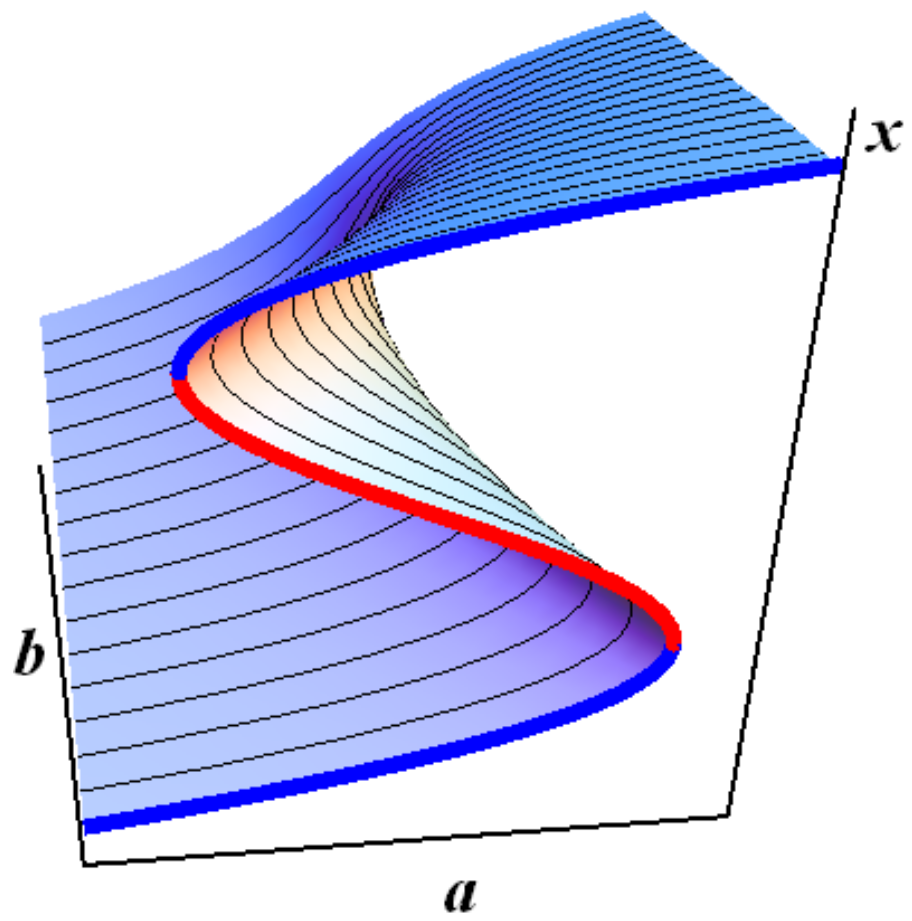
\includegraphics[width=0.95\textwidth]{../Graphics/Bif_Graphs/Bif_3D.png}}
	{These plots show the mentioned co-dimension 2 cusp bifurcation, composed of two co-dimension 1 fold bifurcations.
	The plot on the right is the surface plot of this same model \parencite{weymiens_bifurcation_2014}.}
	{fig:Bif_hysteresis}

\end{frame}

%--------------------------------------

\begin{frame} % Co-dimension 3
\frametitle{Bifurcation Theory}

\begin{figure}[tb] % Co-dimension 3 bifurcation cross-section
\begin{minipage}{0.59\linewidth}
	\centering
	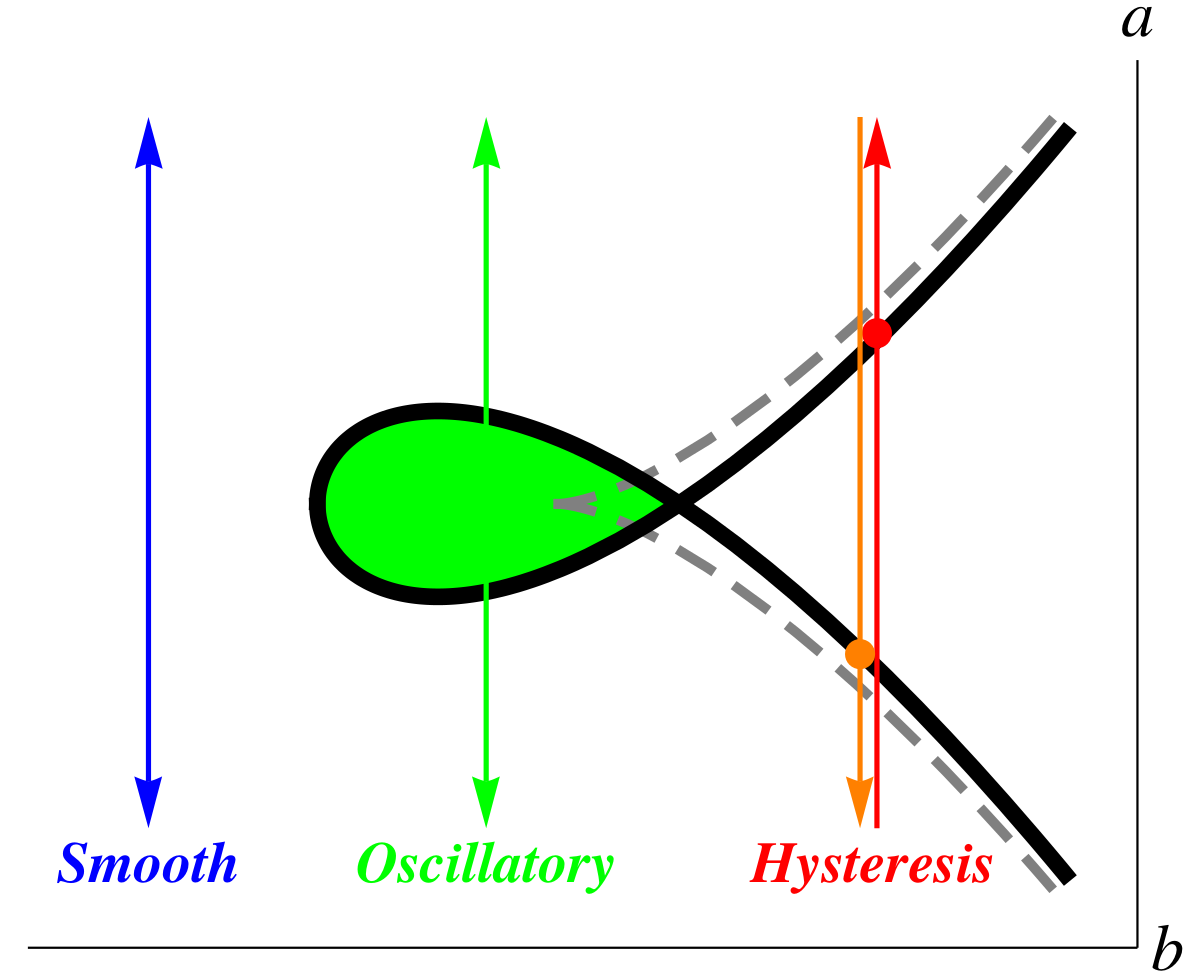
\includegraphics[width=\textwidth]{../Graphics/Bif_Graphs/3_transitions_single_simple.png}
\end{minipage}
\hfill
\begin{minipage}{0.39\linewidth}
	\caption{FitzHugh-Nagumo model, a co-dimension 3 bifurcation with the black line indicating the fold bifurcation.
	It accurately describes the L--H transition in tokamak plasmas, with the $b$ parameter dictating the type of transition \parencite{weymiens_bifurcation_2014}.}
	\label{fig:co-3}
\end{minipage}
\end{figure}

\end{frame}

%--------------------------------------

\section{H--mode}
\begin{frame} % First H--mode slide
\frametitle{H--mode}

\begin{itemize}
	\item The L--H transition is a bifurcation of anomalous transport at the edge. High auxiliary power develops strong sheared $\mathbf{E}\times\mathbf{B}$-drift plasma flow \parencite{terry_suppression_2000}.
	\item Experiments at TEXTOR showed that a biased probe produced H--mode \parencite{weynants_confinement_1992}.
\end{itemize}

\begin{figure}[tb] % L--H-modes compare
\begin{minipage}{0.59\linewidth}
	\centering
	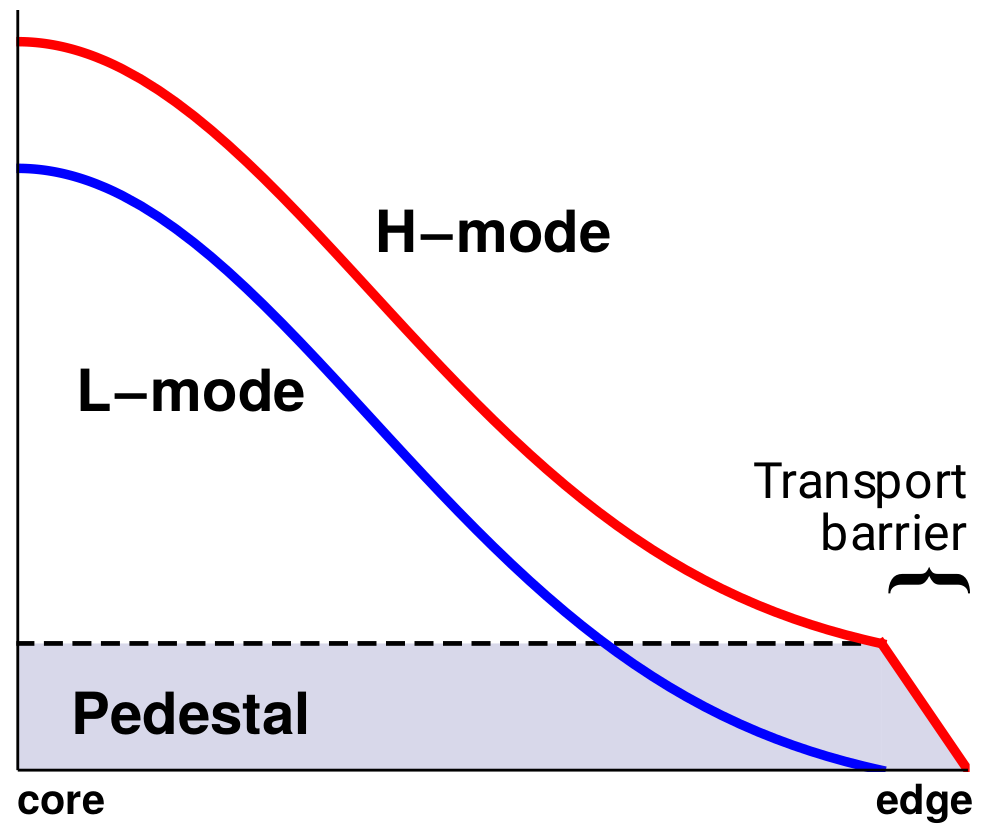
\includegraphics[width=0.75\textwidth]{../Graphics/L-mode_H-mode_compare.png}
\end{minipage}
\hfill
\begin{minipage}{0.39\linewidth}
	\caption{A comparison of the radial pressure profiles of L--mode and H--mode \parencite{weymiens_bifurcation_2014}.}
	\label{fig:L-mode_H-mode_compare}
\end{minipage}
\end{figure}

\end{frame}

%--------------------------------------

\begin{frame} % Radial Electric Field
\frametitle{Radial Electric Field}
\begin{equation} % Lorentz Force Balance
	E_r \,=\, -\frac{1}{n_j e_j} \frac{\text{d} p_j}{\text{d} r} + V_{\theta j} B_\phi - V_{\phi j} B_\theta
	\label{eq:E_r}
\end{equation}
\begin{itemize}
	\item $V_{\theta j}$ and $V_{\phi j}$ are unreasonably-difficult to measure.
	\item Instead, look at nonambipolar particle fluxes that can be calculated by the electric field, density, temperature, and their gradients.
\end{itemize}
\begin{align} % Ambipolarity constraint
	\epsilon_0 \frac{\partial E_r}{\partial t} \,=\, -\sum J_r \,=\,
		\sum_\text{k} q_j\Gamma_j^\text{k} \label{eq:ambipolarity_constraint}
\end{align}
\begin{itemize}
	\item It is useful to normalize the field to the gyroradius and temperature.
\end{itemize}
\begin{align} % Z definition
	Z \,\equiv\, \frac{\rho_{\theta i} \, e \, E_r}{T_i}~, ~~~~
		\rho_{\theta i} \,\equiv\, \frac{m_i \, v_{T_i}}{e \, B_\theta}
		\label{eq:Z_and_rho_definitions}
\end{align}
\end{frame}

%--------------------------------------

\section{Dynamical Model}
\begin{frame} % Transport Equations
\frametitle{Transport Equations}
\begin{itemize}
	\item Conservation of mass
\begin{align} % n continuity
	\frac{\partial n}{\partial t} \,=\, -\frac{\partial \Gamma}{\partial x}~,
		~~~ \Gamma \,=\, -D \, \frac{\partial n}{\partial x}
		\label{eq:n_continuity}
\end{align}
	\item Conservation of energy
\begin{align} % U continuity
	\frac{\partial U}{\partial t} \,=\, -\frac{\partial q}{\partial x}~,~~~
		q \,=\, -\chi \, n \, \frac{\partial T}{\partial x} \,+\,
	\frac{\Gamma \, T}{\gamma - 1}
\end{align}
	\item Particle-Thermal Diffusivity Coupling
\begin{align} % D to chi
	\chi \,=\, \frac{D}{\zeta (\gamma - 1)}~,~~~ \zeta \approx 0.5
\end{align}
	\item Compact Equations
\begin{align} % More reduced temperature equation
	\dot{n} \,=\, \frac{\partial}{\partial x} \left[D \, n^\prime\right]~,~~
	\frac{\partial(n\,T)}{\partial t} \,&=\, \frac{\partial}{\partial x}
		\left[\frac{D\,n}{\zeta} \, T^\prime\right]
		\,+\, \frac{\partial}{\partial x} \left[D\, n^\prime \, T \right]
		\label{eq:U_compact}
\end{align}
\end{itemize}
\end{frame}

%--------------------------------------

\begin{frame} % Nonambipolar fluxes
\frametitle{Nonambipolar Fluxes}
6 different nonambipolar fluxes were included in the investigation.
\parencite{stringer_explanation_1993} \parencite{itoh_role_1996} \parencite{toda_theoretical_1997} \parencite{staps_backstepping_2017} \\
%\begin{columns}[T]
%	\column{0.5\textwidth}
%		Polarization Current \\ Ion Shear Viscosity \\ Ion Bulk Viscosity \\
%		Charge Exchange Friction \\ Anomalous Electron Loss \\ Ion Orbit Loss
%	\column{0.5\textwidth}
%	\begin{align*}
%		J^\text{pol} \propto \dot{Z} \\ J^{\pi\perp} \propto \\ J^{\pi\parallel} \\
%		J^\text{cx} \\ J^\text{an} \\ J^\text{ol}
%	\end{align*}
%\end{columns}
\begin{center}
\begin{tabular}{l|l} \hline
	Polarization Current & $J^\text{pol} \propto \rho_{\theta i}\, n \, \dot{Z}$ \\ \\
	Ion Shear Viscosity & $J^{\pi\perp} \propto \rho_{\theta i} \,
		\nabla\left[\mu \, n \, Z^\prime\right]$ \\ \\
	Ion Bulk Viscosity$\dagger$ & $J^{\pi\parallel} \propto \rho_{\theta i}
		\left(n\,T^\prime + \frac{n\,T\,Z}{\rho_{\theta i}}\right)
		\exp\left[-Z^2 + \dotsb\right]$ \\ \\
	Ion Orbit Loss & $J^\text{ol} \propto \rho_{\theta i} \, n \,
		\frac{\exp\left[-\sqrt{Z^4 + \dotsb}\right]}{\sqrt{Z^4 + \dotsb}}$ \\ \\
	Charge Exchange Friction & $J^\text{cx} \propto n_0 \,
		\langle \sigma_\text{cx} v\rangle \left(\nabla (n\,T) +
		\frac{n\,T\,Z}{\rho_{\theta i}}\right)$ \\ \\
	Anomalous Electron Loss & $J^\text{an} \propto \rho_{\theta e}
		\left(\nabla (n\,T) + \frac{n\,T\,Z}{\rho_{\theta i}}\right)$
\end{tabular}
\end{center}
% ----------------- Try again
%\begin{align}
%	\text{Polarization Current:}&~~ J^\text{pol} \,=\, \frac{e \, n \,
%		\rho_{\theta i}}{2} \, \frac{\partial Z}{\partial t}
%		\label{eq:polarization_current_normalized} \\
%	\text{Ion Shear Viscosity:}&~~ J^{\pi\perp} \,=\, -\frac{e \, \rho_{\theta i}}{2} \,
%		\frac{\partial}{\partial x} \left[\mu \, n \, \frac{\partial Z}
%		{\partial x}\right] \label{eq:shear_current_normalized} \\
%	\text{Ion Orbit Loss:}~~ \Gamma_i^\text{ol} \,&=\, n \, \rho_{\theta i} \,
%		\nu_{ii} \, \nu_{*i} \, \frac{\exp\left[-\sqrt{\nu_{*i} + Z^4
%		+ \left(\frac{x}{w_{bi}}\right)^4}\right]}{\sqrt{\nu_{*i} + Z^4
%		+ \left(\frac{x}{w_{bi}}\right)^4}} \label{eq:Gamma_ol}
%	\text{Charge Exchange Friction:}~~ \Gamma_e^\text{cx} \,=\,
%		-\frac{m_i \,n_0 \langle\sigma_\text{cx} v\rangle \, n\,T}{B_\theta^2}
%		\, \left[\frac{B_\theta^2}{\epsilon^2 B_\phi^2} + 2\right] \,
%		\left(\frac{n^\prime}{n} \,+\, \frac{\alpha_\text{cx}\,T^\prime}
%		{T} + \frac{Z}{\rho_{\theta i}}\right) \label{eq:Gamma_cx} \\
%	\text{Anomalous Electron Loss:}~~ \Gamma_e^\text{an} \,=\, -n_e \,
%		D_\text{an} \left(\frac{n^\prime}{n} \,+\,
%		\frac{\alpha_\text{an}\,T_e^\prime}{T_e} \,+\,
%		\frac{e\,E_r}{T_e}\right) \label{eq:Gamma_an_orig} \\
%	D_\text{an} \,=\, \frac{\epsilon^2 \sqrt{\pi}}{2 a_m}
%		\frac{\rho_{\theta e} \, T_e}{B} \label{eq:D_an} \\
%	\text{Ion Bulk Viscosity:}~~ \Gamma_i^{\pi\parallel} \,=\, \,n_e\,D_{\pi\parallel}
%		\left(\frac{n^\prime}{n} + \frac{Z}{\rho_{\theta i}}\right) \,
%		\text{Im}\left[X\left(Z \,+\, i\,\frac{\nu_{ii}}{\omega_t}\right)\right]
%		\label{eq:stringer_Gamma_bulk} \\
%\end{align}
\end{frame}

%--------------------------------------

\begin{frame} % Z equations
\frametitle{Radial Electric Field Equations}

Flux model
\begin{align} % Flux model
	\epsilon_0 \frac{\partial E_r}{\partial t} \,&=\, -\sum_\text{k} J^\text{k} \\
	\frac{e \, n \, \rho_{\theta i}}{2} \, \frac{\partial Z}{\partial t}
		\,&=\, \frac{e \, \rho_{\theta i}}{2} \frac{\partial}{\partial x}
		\left[\mu \, n \, \frac{\partial Z}{\partial x}\right] \,-\,
		J^{\pi\parallel} \,+\, J^\text{an} \,-\, J^\text{cx} - J^\text{ol}
		\label{eq:normalized_Z_equation}
\end{align}

Taylor-expanded model \parencite{zohm_dynamic_1994}
\begin{align} % Taylor-expanded model
	\epsilon \, \frac{\partial Z}{\partial t} \,=\, \mu \,
		\frac{\partial^2 Z}{\partial x^2} \,+\, \frac{c_n T}{n^2} \,
		\frac{\partial n}{\partial x} \,+\, \frac{c_T}{n} \,
		\frac{\partial T}{\partial x} \,+\, G(Z)~,\label{eq:original_Z_equation} \\
	G(Z) \,\equiv\, a \,+\, b(Z - Z_S) \,+\, c(Z - Z_S)^3
		\label{eq:G_polynomial}
\end{align}

\end{frame}

%--------------------------------------

\begin{frame} % Diffusivities and Boundary Conditions
\frametitle{Diffusivity Model and Boundary Conditions}

The particle diffusivity must be dependent on both the field and its shear \parencite{paquay_studying_2012}.
\begin{align} % Flow-Shear diffusivity
	D(Z, Z^{\prime}) \,=\, D_\text{min} \,+\,
		\frac{D_\text{max} - D_\text{min}}{1 \,+\, a_1 Z^2 \,+\,
		a_3 (Z^{\prime})^2} \label{eq:flow_shear_diffusivity}
\end{align}

Boundary conditions can dictate overall behavior
\begin{align} % All boundary conditions
	\Gamma(L) \,&=\, \Gamma_c~,~~~ &q(L) \,=\, q_c~,~~~ Z^\prime(L) \,&=\, 0 \\
	n^\prime(0) \,&=\, \frac{n}{\lambda_n}~, ~~~~ &T^\prime(0) \,=\,
	\frac{T}{\lambda_T}~,~~~ Z^\prime(0) \,&=\, \frac{Z}{\lambda_Z} ~~
		\text{or} ~~ Z^\prime(0) \,=\, 0
\end{align}

\end{frame}

%--------------------------------------

\section{Results}
\begin{frame} % State plot
\frametitle{Taylor-Expanded Model}

\begin{figure}[h]
\begin{minipage}{0.65\linewidth}
	\centering
	\includegraphics[width=\textwidth]{../Graphics/Model_Graphs/Original_FS_0135.png}
\end{minipage}
\begin{minipage}{0.34\linewidth}
	\caption{H--mode, with a clear transport barrier, using the Flow-Shear model of diffusivity.}
\end{minipage}
\end{figure}
\end{frame}

\begin{sagesilent}
	reset()

	var('Z')

	c_n, c_T = -1.1, -0.9
	a, b, c = 3.0/2.0, 2.0, -1.0
	Z_S = -3.0/2.0

	# At t = 0
	#0.49	0.683706980466396	1.32496145938483	-0.0206250867984561	5
	#0.51	0.691213814264995	1.33027412776876	-0.0191672209048899	5
	#0.53	0.698719562491543	1.33554223315998	-0.0177733476721204	5

	# At t = 135
	#0.49	0.610660563155032	1.30411254952973	-3.06036908428267	2.66118461102601
	#0.51	0.618549890710752	1.31299641246706	-3.05151915868033	2.66386371895
	#0.53	0.626467999984115	1.32173998954979	-3.0425333319374	2.66544015688424
	# .........
	#0.99	0.981110868143376	1.63421628926577	-1.48108678379191	0.491444796219089
	#1.01	0.999673727872353	1.64981311266731	-1.28285663026662	0.499537912103461
	#1.03	1.01660486587383	1.66401200235489	-1.09300528560897	0.513478891305364
	# .........
	#1.99	1.2435198107485	1.79762273772508	0.141694442025275	4.9908892834125
	#2.01	1.24801940647034	1.79934360213636	0.141647858350999	4.99089991282975
	#2.03	1.2525541146463	1.80107077486164	0.141626086988019	4.99090015667972

	t = (0, 135, 135, 135)
	x = (0.51, 0.51, 1.01, 2.01)
	density = (0.691213814264995, 0.618549890710752, 0.999673727872353, 1.24801940647034)
	density_grad = ((0.698719562491543 - 0.683706980466396) / 0.04,\
			(0.610660563155032 - 0.626467999984115) / 0.04,\
			(1.01660486587383 - 0.981110868143376) / 0.04,\
			(1.2525541146463 - 1.2435198107485) / 0.04)
	temperature = (1.33027412776876, 1.31299641246706, 1.64981311266731, 1.79934360213636)
	temperature_grad = ((1.33554223315998 - 1.32496145938483) / 0.04,\
			(1.32173998954979 - 1.30411254952973) / 0.04,\
			(1.66401200235489 - 1.63421628926577) / 0.04,\
			(1.80107077486164 - 1.79762273772508) / 0.04)

	colors = rainbow(len(x) + 1)

	G(Z) = a + b*(Z - Z_S) + c*(Z - Z_S)^3

	steady_state_plots = []

	for j in range(len(x)):
	    f(Z) = (c_n * temperature[j] / density[j]^2) * density_grad[j] + (c_T / density[j]) * temperature_grad[j] + G(Z)
	    steady_state_plots.append(plot(f, (Z,-3.5,1.5), ymin=-3, ymax=4,\
	    		gridlines=True, color=colors[j], axes_labels=["$Z$",""],\
	    		thickness=2.0, legend_label="$x = " +str(x[j].n(digits=3))\
	    		+"$, $t = " +str(t[j].n(digits=3))+ "$"))

	steady_state_plots.append(plot(G, (Z,-3.5,1.5), gridlines=True,\
			color=colors[-1], thickness=2.0, legend_label="$G(Z)$"))

	equation_label = text(r"$f(Z) = \frac{c_n \, T}{n^2} \, \frac{\partial n}{\partial x} \,+\, \frac{c_T}{n} \, \frac{\partial T}{\partial x} \,+\, G(Z)$",\
			(-2,-2.5), bounding_box={'boxstyle': 'round', 'fc': 'w'},\
			fontsize=16, color='black')

	combined_plots = sum(steady_state_plots) + equation_label
	combined_plots.set_aspect_ratio(0.4)
\end{sagesilent}
\begin{frame} % Show zeros
\frametitle{Taylor-Expanded Model}
\begin{figure}[h]
	\sageplot[width=0.9\textwidth]{combined_plots}
	\caption{The steady-state values across $Z$ at different locations in the domain.
	Also, the first time step and the polynomial $G(Z)$ are added for comparison.}
\end{figure}
\end{frame}

%--------------------------------------

\begin{frame} % Pre-oscillations
\frametitle{Flux Model}
\TwoFigOneCap{\includegraphics[width=\linewidth]{../Graphics/Model_Graphs/state_G1e20_full_t200.png}}
	{\includegraphics[width=\linewidth]{../Graphics/Model_Graphs/flux_G1e20_full_t200.png}}
	{$Z^\prime(0) = Z / \lambda_Z$ used, causing the initial decrease in diffusivity at the edge.}
	{fig:flux_state_full}
\end{frame}


\begin{frame} % The steady-state pre-oscillation
\frametitle{Flux Model}
\begin{figure}[!b] % Fluxes vs Z, SAVED IMAGE, because it's too much code
	\centering
	\includegraphics[width=0.9\textwidth]{../Graphics/Model_Graphs/Fluxes_vs_Z_core_t200.png}
	\caption{Steady-state. The anomalous electron loss and charge exchange friction are nearly identical.
	The blue vertical line indicates the true value of $Z$.}
	\label{fig:fluxes_steady-state}
\end{figure}
\end{frame}


\begin{frame} % Temporary H--mode
\frametitle{Flux Model}
\TwoFigOneCap{\includegraphics[width=\textwidth]{../Graphics/Model_Graphs/state_G1e21_full_t190.png}}
	{\includegraphics[width=\textwidth]{../Graphics/Model_Graphs/flux_G1e21_full_t190.png}}
	{Higher core fluxes ($\Gamma_c = 10^{21}~\text{m}^{-2}\cdot\text{s}^{-1}$), the system makes a transition.}
	{fig:higher_core_flux}
\end{frame}


\begin{frame} % Oscillations
\frametitle{Flux Model}

\TwoFigOneCap{\includegraphics[width=\textwidth]{../Graphics/Model_Graphs/state_G1e20_extended_t1059.png}}
	{\includegraphics[width=\textwidth]{../Graphics/Model_Graphs/state_G1e20_extended_t1060.png}}
	{It has been zoomed in to 6 mm inside of the plasma edge to showcase the unexplained oscillations, with a frequency still comparable to the time step.}
	{fig:oscillations_extended}

\end{frame}


\begin{frame} % No steady-state
\frametitle{Flux Model}

\begin{figure}[tb] % Fluxes vs Z for 40000
	\centering
	\includegraphics[width=0.9\textwidth]{../Graphics/Model_Graphs/Fluxes_vs_Z_oscillations_t40000.png}
	\caption{The fluxes as a function of $Z$ in the center of the oscillations a long-term run.
	The vertical blue line indicates the actual value of $Z$; since it is nowhere near a zero, this particular point in the domain is not at steady-state.}
	\label{fig:fluxes_steady-state_40000}
\end{figure}

\end{frame}

%--------------------------------------

\section{Conclusions} % and ending
\begin{frame} % Conclusions
\frametitle{Conclusions and Future}

\begin{itemize}
	\item H--mode can be generated, but not as steady-state.
	\item No dithering phase observed.
	\item $J^{\pi\parallel}$ consistently has the largest effect; $J^\text{an}$ comes in second.
	\item $J^\text{ol}$ becomes insignificant in the presence of a nonzero field, therefore cannot be dominant.
\end{itemize}
\hrule
\begin{itemize}
	\item $J^\text{cx}$ has more chosen (rather than) parameters; more analytic model should be used.
	\begin{itemize}
		\item It is also most closely related to the input power by definition of $n_0$, also doesn't account for different species of neutrals.
	\end{itemize}
	\item Bifurcation analysis needed on the sum of fluxes to prove it has needed characteristics.
	\item `Unrealistic' oscillations and lack of consistent steady-state hinder any further progress.
\end{itemize}

\end{frame}

%--------------------------------------

%\section{References}
\begin{frame}
\frametitle{References}
\renewcommand*{\bibfont}{\tiny}
%\nocite{*}
\printbibliography
\end{frame}

%-------------------------------------- EXTRAS!

\appendix
\begin{frame} % J^pol, J^shear, J^bulk
\begin{align}
	J^\text{pol} \,&=\, \frac{e \, n \, \rho_{\theta i}}{2} \,
		\frac{\partial Z}{\partial t} \\
	J^{\pi\perp} \,&=\, -\frac{e \, \rho_{\theta i}}{2} \,
		\frac{\partial}{\partial x} \left[\mu \, n \, \frac{\partial Z}
		{\partial x}\right] \\
	J^{\pi\parallel} \,&=\, e\,n_e\,D_{\pi\parallel}
		\left(\frac{n^\prime}{n} + \frac{Z}{\rho_{\theta i}}\right) \,
		\text{Im}\left[X\left(Z \,+\, i\,\frac{\nu_{ii}}{\omega_t}\right)
		\right] \\
	&D_{\pi\parallel} \,=\, \frac{\epsilon^2\,\rho_{\theta i}\,T}
		{(x - a_m)\sqrt{\pi}\,B} \\
		X(z) \,&\equiv\, i\,\sqrt{\pi} \, \exp(-z^2) \, \text{erfc}(-i\,z) \,=\,
		\frac{1}{\sqrt{\pi}} \int_{-\infty}^{+\infty} \frac{e^{-t^2}}{t - z}
		\, \text{d}t
\end{align}
\end{frame}

\begin{frame} % Last 3 fluxes
\begin{align}
	J^\text{an} \,&=\, -e \, n_e \, D_\text{an} \left(\frac{n^\prime}{n}
		\,+\, \frac{\alpha_\text{an}\,T_e^\prime}{T_e} \,+\,
		\frac{Z}{\rho_{\theta i}}\right) \\
	&D_\text{an} \,=\, \frac{\epsilon^2 \sqrt{\pi}}{2 a_m}
		\frac{\rho_{\theta e} \, T_e}{B} \\
	&n_0 \,\propto\, \frac{\Gamma_c}{v_{T_i}\left[1 \,+\,
		\exp{(k(x - d))}\right]} \\
	J^\text{cx} \,&=\,
		-\frac{m_i \,n_0 \langle\sigma_\text{cx} v\rangle \, n\,T}{B_\theta^2}
		\, \left[\frac{B_\theta^2}{\epsilon^2 B_\phi^2} + 2\right] \,
		\left(\frac{n^\prime}{n} \,+\, \frac{\alpha_\text{cx}\,T^\prime}
		{T} + \frac{Z}{\rho_{\theta i}}\right) \\
	J^\text{ol} \,&=\, e \, n \, \rho_{\theta i} \, \nu_{ii} \, \nu_{*i} \,
		\frac{\exp\left[-\sqrt{\nu_{*i} + Z^4
		+ \left(\frac{x}{w_{bi}}\right)^4}\right]}{\sqrt{\nu_{*i} + Z^4
		+ \left(\frac{x}{w_{bi}}\right)^4}}
\end{align}
\end{frame}

\begin{frame}
\centering
Are the oscillations ELMs? \\
\Huge No
\end{frame}

\begin{frame} % Super long-term state

\begin{figure}[h]
\begin{minipage}{0.69\linewidth}
	\includegraphics[width=\textwidth]{../Graphics/Model_Graphs/state_G1e20_extended_t40000.png}
\end{minipage}
\begin{minipage}{0.29\linewidth}
	\caption{After 20 ms, oscillations still dominate, with the domain of oscillation increased in size.}
\end{minipage}
\end{figure}

\end{frame}

\end{document}

